\documentclass[a4paper, 11pt]{report}
\usepackage[utf8]{inputenc} 
\usepackage[T1]{fontenc}
\usepackage[frenchb]{babel} %ou \usepackage[francais]{babel} 
\usepackage{url} %écrire des adresses cliquables
\usepackage{lmodern} %changer pack de police
\usepackage[top=3cm, bottom=3cm, left=3cm, right=3cm]{geometry} %gérer les marges
\usepackage{color}
\usepackage[babel=true]{csquotes} % csquotes va utiliser la langue définie dans babel
\usepackage{graphicx}
\usepackage[space]{grffile}
\usepackage{listings}
\lstset{language=C,basicstyle=\small,frame=leftline,captionpos=b,linewidth=175mm,breaklines=true, ,identifierstyle=\ttfamily, numbers=none, numberstyle=\tiny, stepnumber=5, numberfirstline=true, showstringspaces=false}
%\input{milstd}
\DeclareGraphicsExtensions{.jpeg, .png , .gif, .bmp}
%\usepackage{eurosym}
\usepackage{array}
\newcolumntype{M}[1]{>{\raggedright}m{#1}}
\usepackage{wrapfig}


%%%%%%%%%%%%%%%%%%%%%%%%%
\begin{document}


% placement des elements
\makeatletter
	\def\clap#1{\hbox to 0pt{\hss #1\hss}}%
	\def\ligne#1{%
	\hbox to \hsize{%
	\vbox{\centering #1}}}%
	\def\haut#1#2#3{%
	\hbox to \hsize{%
	\rlap{\vtop{\raggedright #1}}%
	\hss
	\clap{\vtop{\centering #2}}%
	\hss
	\llap{\vtop{\raggedleft #3}}}}%
	\def\bas#1#2#3{%
	\hbox to \hsize{%
	\rlap{\vbox{\raggedright #1}}%
	\hss
	\clap{\vbox{\centering #2}}%
	\hss
	\llap{\vbox{\raggedleft #3}}}}%
	\def\maketitle{%
	\thispagestyle{empty}\vbox to \vsize{%
	\haut{}{\@blurb}{}
	\vfill
	\vspace{1cm}
\begin{flushleft}
	%\usefont{OT1}{ptm}{m}{n}
	\huge \@title
\end{flushleft}
	\par
	\hrule height 4pt
	\par
\begin{flushright}
	%\usefont{OT1}{phv}{m}{n}
	\Large \@author
	\par
\end{flushright}
	\vspace{1cm}
	\vfill
	\vfill

\begin{center}
	
\includegraphics[width=7cm]{logo_UTBM2.jpg}
\end{center}

\bas{}{Printemps 2013}{}
}%
\cleardoublepage
}
\def\date#1{\def\@date{#1}}
\def\author#1{\def\@author{#1}}
\def\title#1{\def\@title{#1}}
\def\location#1{\def\@location{#1}}
\def\blurb#1{\def\@blurb{#1}}
\date{\today}
\author{}
\title{}

% informations
\location{Belfort}\blurb{}
\makeatother
\title{Rapport de projet - Affectation des fréquences dans les réseaux mobiles}
\author{\small{Thomas Gloriod, Paul Locatelli et Pierre Rognon}}
\blurb{%
	\textbf{AG41 - Optimisation et recherche opérationnelle}\\
	Université de Technologie de Belfort-Montbéliard
}% 


\maketitle
\tableofcontents 
%%%%%%%%

\chapter{Introduction}
Afin de clore l'étude concernant l'optimisation et la recherche opérationnelle, un projet a été proposé. Ce projet concerne l'affectation de fréquences dans le cadre d'antennes pour les réseaux mobiles. L'enjeu réside dans le fait que cette affectation se joue sur un carte qui est familière ici puisque l'on se concentrera sur le Territoire de Belfort.\\
Le problème d'affectation de fréquences est un problème type en recherche opérationnelle. Il est donc connu de tous les initiés de cette discipline.\\
Plus précisément, ce problème s'apparente à un problème de coloration de graphe. Il s'agit ici d'attribuer des fréquences à différents secteurs d'une même zone. La contrainte consiste à éviter le plus possible que deux secteurs limitrophes émettent sur la même fréquence.\\
La modélisation de ce problème représentant un travail important, le projet consiste seulement à se pencher sur la méthode de résolution. Une première partie consiste donc à trouver une solution initiale, c'est-à-dire affecter une première fois les fréquences sans se préoccuper outre mesure de l'efficacité de cette affectation. La seconde partie consiste à améliorer cette affectation en proposant des solutions plus efficaces à l'aide d'un algorithme de notre choix. Ici, le choix s'est porté sur un algorithme de recherche tabou.

\chapter{Présentation du sujet}

	\section{Détails du problème}
	Le département étudié, ici le Territoire de Belfort comporte 36 secteurs, chacun étant divisé en maximum trois secteurs. On obtient ainsi un total de 88 secteurs. Trois fréquences sont disponibles pour chaque secteur. Ces fréquences sont donc numérotées 1, 2 et 3 afin de reconna\^itre facilement celle-ci. \\

\begin{center}
	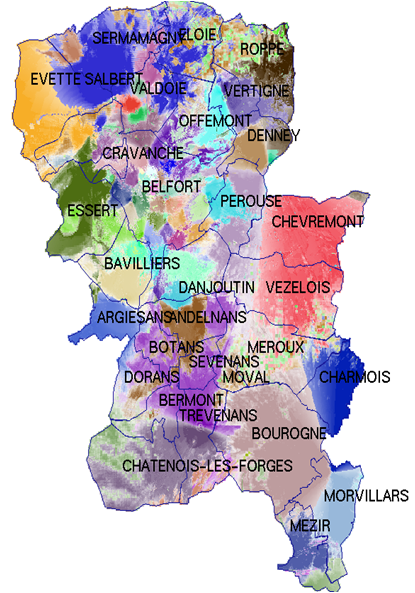
\includegraphics[width=5cm]{carte.png}\\
	\emph{Cette carte représente le territoire qui sera étudié par ce projet soit le département du Territoire de Belfort.\\}
\end{center}

	Chaque secteur reçoit donc dans son affectation  un secteur en fréquence 1, un autre en fréquence 2 et un dernier en fréquence 3. Sur la carte ci-dessous, on peut voir l'agencement théorique de sites entre eux ainsi que la division en secteurs de ceux-ci.
	
	\begin{center}
		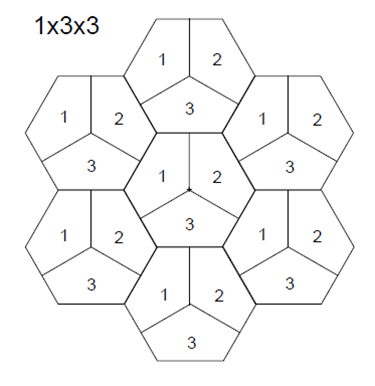
\includegraphics[width=5cm]{ruche}\\
		\emph{Chaque site est délimité en trois secteurs ici identiques mais qui peuvent en réalité varier et ont des frontières plus floues.\\}
	\end{center}

Pour que les clients soient couvert, les secteurs ayant une frontière communes doivent avoir des fréquences différentes afin de minimiser les interférences.\\
Cependant, il n'est pas aisé de savoir si des clients observent des interférences. C'est pourquoi, au sein du territoire, 12 695 points test permettent d'évaluer la qualité de l'allocation des fréquences. Chaque points test est caractérisé par un nombre de clients et le débit souhaité pour chacun. 

	\section{Objectifs}

	L'objectif ici se cache derrière un premier objectif d'ordre technique. En effet, il faut tout d'abord réduire au maximum le nombre de fréquences égales qui se chevaucheraient. Par le chevauchement, on entend une frontière entre deux secteurs, de sites différents, affectés à la même fréquence.\\
	Cependant, derrière cet objectif, le fait de minimiser les conflits, un autre objectif final se cache. Chaque interférence générée par un conflit génère en effet une zone dans laquelle le signal risque fortement d'\^etre perturbé et d’empêcher l'utilisation d'un téléphone par un client potentiel. C'est donc ce problème que l'on cherche à minimiser.


\chapter{Principe de résolution}
	
	La résolution de ce problème peut se faire de deux façons totalement différentes. La première est de manière exacte. L'utilisation de méthode exacte demanderait le calcul de 6\up{36} soit environ 10\up{28} allocation de fréquences différentes. Le temps de calcul n'est donc pas réalisable aujourd'hui, les ordinateurs actuels n'étant pas assez puissants. C'est pourquoi pour ce genre de problème ou le nombre de solution est trop importante, les méthode de résolution approchée sont utilisées.

		\section{Le choix d'une méthode approchée}
		Le principe de cette méthode de résolution est simple. On cherche d'abord une solution au problème, soit de manière aléatoire, soit en en calculant pas trop mauvaise.
		Une liste de voisins à cette solution est ensuite définie. Les voisins sont alors issus de règles précises définies auparavant suivant la méthode approchée à utiliser.
		Il faut ensuite évaluer tous ces voisins afin d'améliorer la solution si possible. La réitération de cette méthode un grand nombre de fois permet de balayer de nombreuses solutions et d'approcher voire de trouver la solution optimale.\\
		L'avantage de ces méthodes approchées est qu'à défaut d'être certain de trouver à coup sûr la bonne solution, il est toujours possible de trouver une solution dont on peut se satisfaire et ce, de manière beaucoup plus rapide que pour une méthode exacte.\\
		Parmi les méthodes approchées, un choix a dû être fait pour ce projet. Ce choix s'est porté sur l'algorithme de la recherche tabou.

		\section{La recherche tabou}
		L'algorithme de recherche tabou permet d'améliorer une simple recherche du meilleur voisin (méthode du hill climbing). En effet, si l'on recherche simplement le meilleur voisin à chaque itération, il est possible quel l'algorithme bloque sur un extremum local. Si la solution n'a que des voisins plus mauvais, l'algorithme va donc considérer que c'est la meilleure solution, même si une solution plus intéressante est disponible.\\
		La recherche tabou permet d'éviter de bloquer dans la plupart des extremums locaux. Cela paraissait donc un choix intéressant dans le cas de l'affectation de fréquences. En effet, le nombre de solution étant relativement important, il est très fortement probable que des extremums locaux existent. L'utilisation de la recherche tabou va éviter de rester bloquer dans un extremum et ainsi d'explorer plus de solutions dans un même nombre d'itérations. Le principe de recherche des voisins de la recherche tabou étant similaire au hill climbing, peu de modifications sont nécessaires. Il suffit, lorsqu'une solution voisine est étudiée, de la placer dans une liste "tabou". On lui attribue alors une durée tabou qui va permettre d'indiquer le nombre d'itérations durant lequel il sera interdit de retourner sur la solution. La liste tabou va donc enregistrer toutes les solutions actuellement interdites ainsi que la durée restante. Dans le cas où une solution présente dans la liste tabou est un extremum local, on évitera ainsi d'y retourner et l'on pourra s'en éloigner.

\chapter{Algorithme développé}

	Comme déjà abordé précédemment, deux partie ont été nécessaires pour pouvoir générer une solution optimale. La première partie consiste à générer une première solution, la seconde à l'améliorer.

	\section{Génération de la solution initiale}
	
	Pour la recherche d'une première solution, la démarche s'est effectuée en plusieurs étapes. La première consistait à lister les méthodes possibles, la seconde à l'implémenter et enfin la dernière à l'évaluer afin de savoir s'il est possible de s'en satisfaire.\\
	La première méthode possible, la plus évidente aussi, est le choix d'une solution aléatoire. Dans ce cas, aléatoire signifie une attribution de la fréquence 1, 2 ou 3 aux secteurs d'un site de façon non redondante, mais sans se préoccuper des autres sites.\\
	Une fois les paramètres de cette méthode choisi, l'algorithme a été implémenté dans le logiciel afin de tester la méthode. Le code de l'algorithme est disponible en annexe 1.\\
	La fonction en annexe est appelée pour chaque sites. Ainsi, à chaque fois, le but est de créer un tableau de taille 3. Chaque case du tableau est remplie par un chiffre, soit 0, soit 1, soit 2. Ces trois chiffres permettent de donner un indice et donc une fréquence à chacun des trois secteurs d'un site.\\
	Pour cela, on va créer deux tableaux, un destiné à être retourné, un autre qui va servir de support. Ce dernier reçoit les trois fréquences à allouer. A chaque fois, on prend aléatoirement une case de ce tableau et on la recopie dans le tableau à retourner.  Cette case est alors supprimée du tableau pour éviter la redondance de fréquence sur le même secteur. En répétant cette opération, on peut retourner un tableau généré de façon aléatoire avec une fréquence affectée à chaque case.\\
	L'appel de cette fonction pour chaque secteur actif permet de construire un tableau complet avec une affectation de fréquences totalement aléatoire.\\
	Après avoir implémenté cette méthode, il est apparu que la fitness correspondante à la solution aléatoire générée était tout à fait satisfaisante. Il a donc été choisi de la garder.
	
	\section{Optimisation de la solution}
	
	Une fois un première solution trouvée, le travail consiste à l'améliorer du mieux possible. Comme indiqué plus en amont dans ce rapport, l'algorithme d'optimisation choisi est la recherche tabou.
	
	
\section{Implémentation de la recherche tabou}

\chapter{Résultats observés}

\chapter{Problèmes rencontrés}

\chapter{Conclusion}
L'algorithme de recherche tabou est fonctionnel. Il permet d'obtenir une fitness très satisfaisante afin d'offrir aux clients la meilleur couverture réseau.

Des améliorations restent possibles en modifiant la méthode du choix des voisins à chaque itération, ou en modifiant la durée de la liste tabou.\\

L'exercice est intéressant car il demande de s'immiscer dans un programme déjà existant, de le comprendre afin d'y ajouter les fonctions à développer. C'est un exercice réaliste puisque dans le monde de l'entreprise, les programmes à développer partent rarement de zéro.\\

Ce projet nous a également permis de nous perfectionner dans le langage C++, de découvrir de nouvelles subtilités et d'améliorer notre manière de programmer. Pour partager les sources du programme, l'utilisation d'un logiciel de gestion de version facilite la tâche.\\

Enfin ce projet a été une expérience enrichissante car effectué au sein d'un groupe de trois étudiants. La communication est importante ainsi que la répartition des tâches. Le travail en groupe permet le partage des compétences et des idées. \\

\appendix
\chapter{Génération de la solution initiale}
\begin{lstlisting}
int* site::randomizeTableFreq(){
    int* tableFreq = new int[3];
    int* table = new int[3]; for(int i=0; i<3;i++)table[i]=i+1;
    int* tableTmp = NULL;
    int taille = 3;
    long random;
    bool shift;
    for(int i=0; i<3; i++)
    {
        shift = false;
        random = Random::aleatoire(taille);
        tableFreq[i]=table[random];
        tableTmp = new int[taille-1];
        for(int j=0; j<taille; j++)
        {
            if(j != random){
                if(shift) tableTmp[j-1] = table[j];
                else tableTmp[j] = table[j];
            }
            else{shift=true;}
        }
        delete table;
        table = tableTmp;
        taille--;
    }
    delete tableTmp;
    return tableFreq;
}
\end{lstlisting}

\chapter{Implémentation de la recherche tabou}
\begin{lstlisting}
\end{lstlisting}

\end{document}
